\chapter{Additional Graphs and Tables}
\section{Simulation}

\begin{table}[h!]
	\caption[Ratio of $g^2-1$ of different photon counting schemes to ground truth value]{Ratio of $g^2-1$ of different photon counting schemes to ground truth value  for $\Delta$=1\, pixel/first maximum. \textit{Closest} is \textit{Combination} without considering Noise photons, giving good results in the low noise cases.}
	\label{tab:photonrecon}
	
\begin{tabular}{lllllll}
	\toprule
	 &        Raw &       Threshold &         Combination &      Closest &         MaxL &          PSANA \\
	\midrule
	Low Signal  &  12 / 0.59 &  6.9 / 0.64 &  0.62 / 0.79 &  0.88 / 0.68 &  0.57 / 0.81 &    -0.5 / 0.66 \\
	High Signal &  2.4 / 1.1 &   1.8 / 1.0 &  0.72 / 0.82 &   1.1 / 0.96 &   1.0 / 0.95 &  -0.026 / 0.79 \\
	High Noise  &  9.3 / 0.3 &  8.1 / 0.39 &   1.0 / 0.58 &   1.3 / 0.46 &  0.44 / 0.54 &   -0.37 / 0.45 \\
	\bottomrule
\end{tabular}

\end{table}

\section{Experiment}

\begin{figure}[h!]
	\centering
	\begin{subfigure}[b]{0.45\textwidth}
		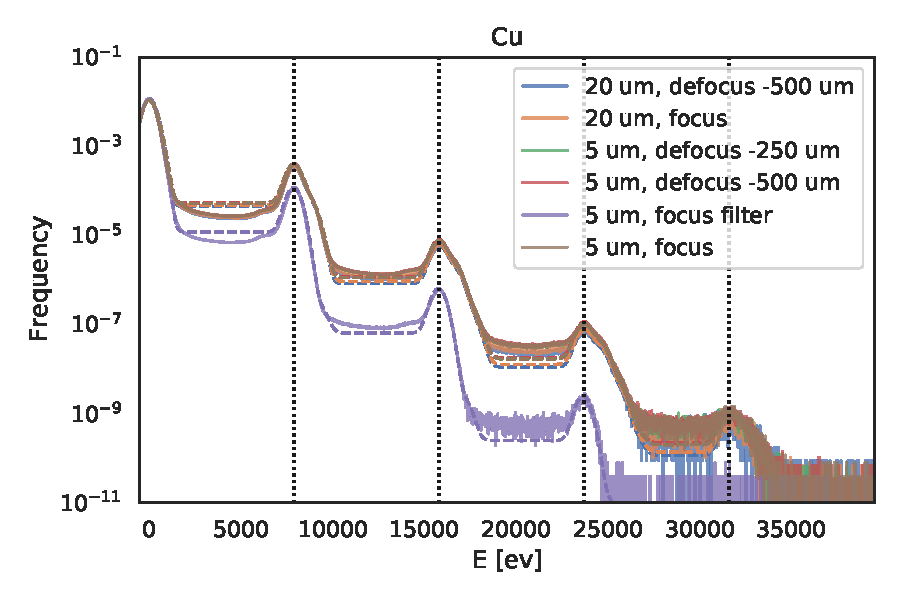
\includegraphics[width=\linewidth]{images/spectrum_foil_cu.pdf}
	\end{subfigure}
	\begin{subfigure}[b]{0.45\textwidth}
		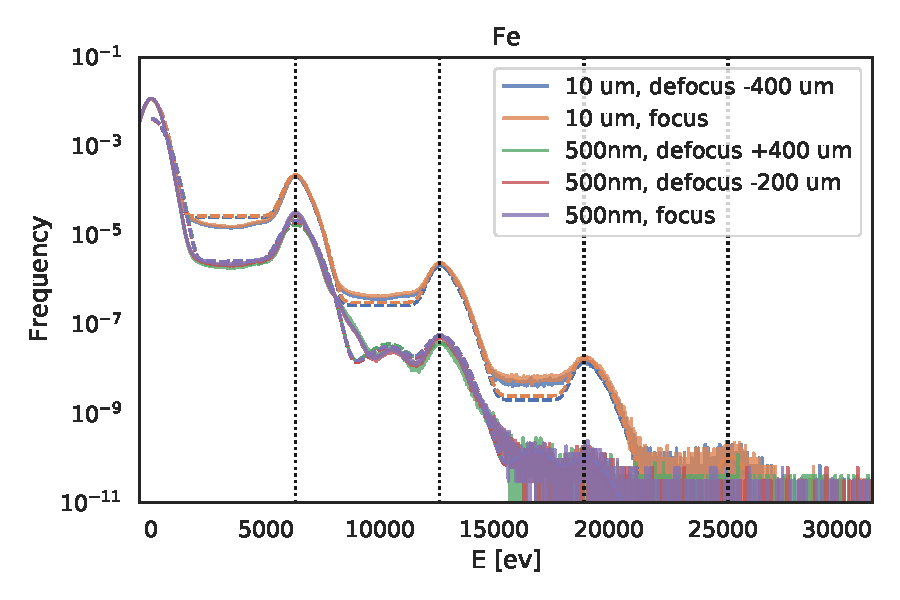
\includegraphics[width=\linewidth]{images/spectrum_foil_fe.pdf}
	\end{subfigure}
	\caption[Spectra of fluorescence using foil samples ]{Spectra of fluorescence using foil samples (left for copper, right for iron) and best fit of the regression.}
	\label{fig:spectrafoil}
\end{figure}

\begin{figure}[h!]
	\centering
	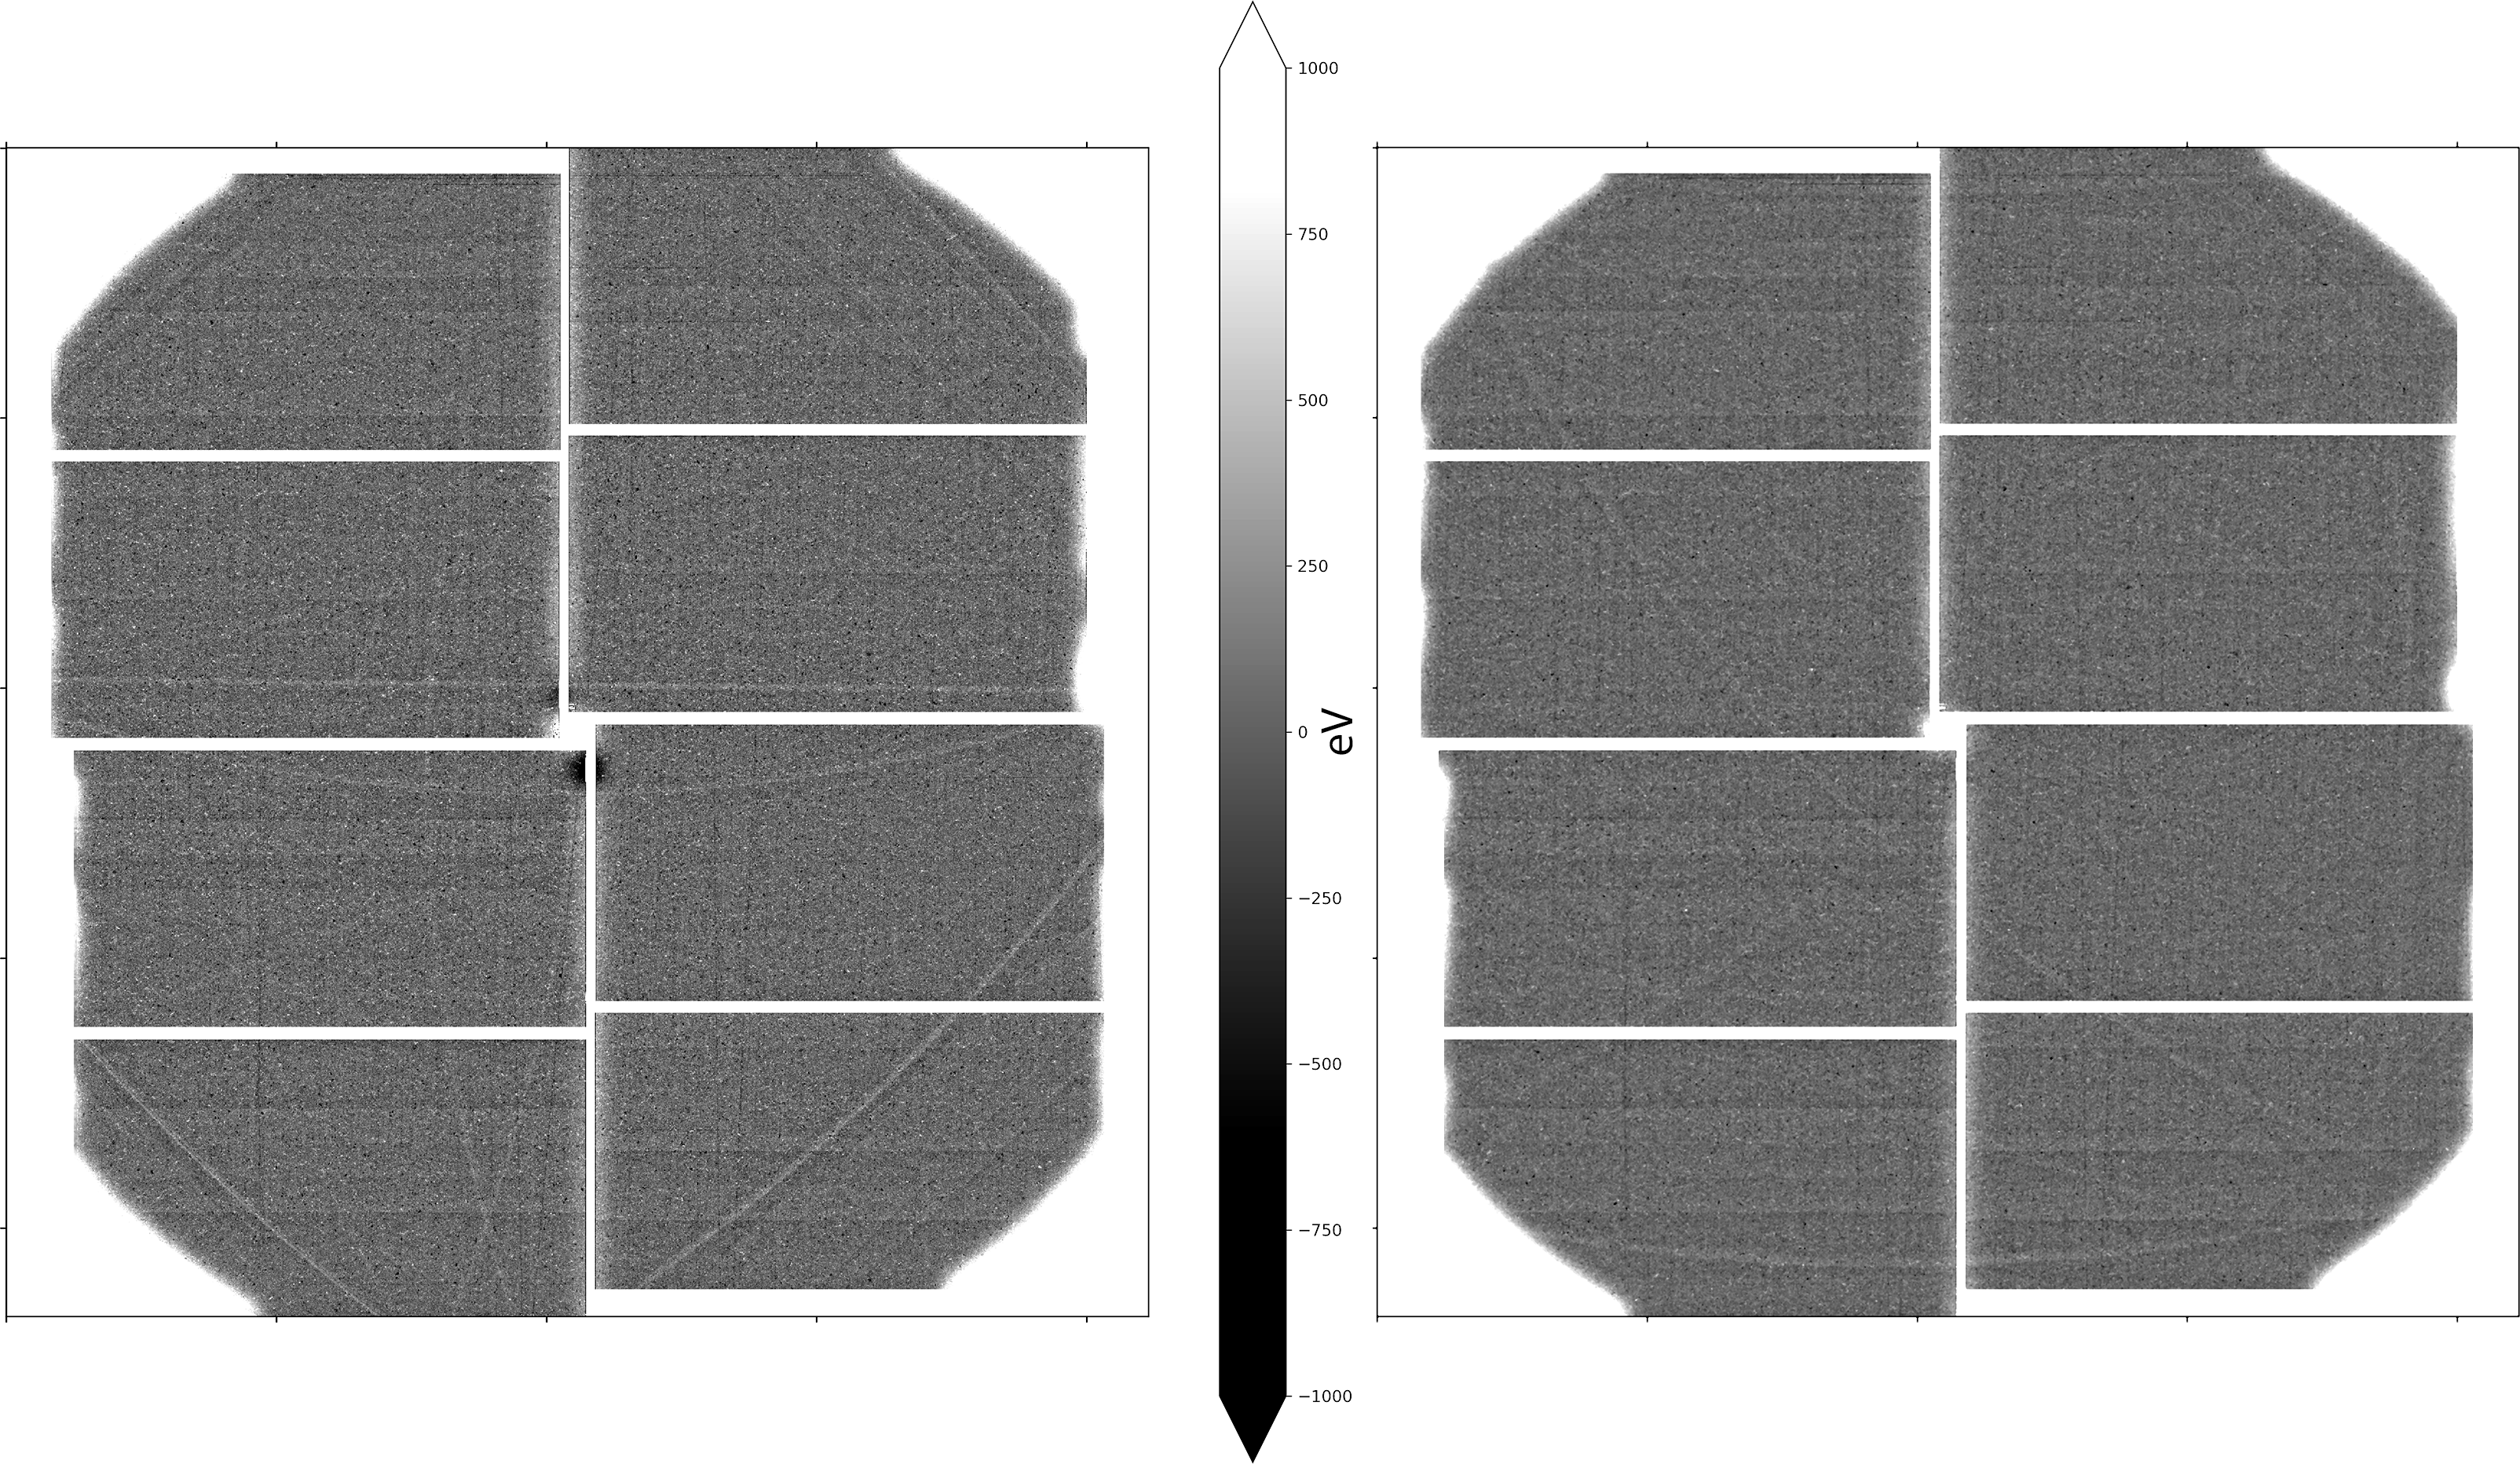
\includegraphics[width=0.8\linewidth]{images/kossel_gaas.png}
	\caption[Mean image of fluorescence of GaAs after background subtraction with visible Kossel lines ]{Mean images of 5000 shots after background subtraction for sample 1 (left) and sample 2 (right), showing the Kossel lines and some artifacts at the edges.}
	\label{fig:kosselgaasmean}
\end{figure}


\begin{table}[h!]
	\caption[Miller Indices considered in Kossel line least squares regression of GaAs sample]{Miller Indices considered in Kossel line least squares regression of GaAs sample 1 (left) and sample 2 (right). Not all possible Kossel lines are visible in the recorded images.}
	\begin{tabular}[t]{lll}
		\toprule
		h&           k &        l \\
		\midrule
	 1 & -1 &  1 \\
	-1 &  1 &  1 \\
	-1 & -1 &  1 \\
	2 & -2 &  0 \\
	-2 &  2 &  0 \\
	-2 & -2 &  0 \\
	2 &  2 &  0 \\
	-3 & -1 &  1 \\
	3 &  1 &  1 \\
	-1 & -3 &  1 \\
	2 & -2 &  4 \\
	-2 & -2 &  4 \\
	2 &  2 &  4 \\
	-2 &  2 &  4 \\
	-4 &  0 &  4 \\
	0 &  4 &  4 \\
	4 &  0 &  4 \\
	0 & -4 &  4 \\
				\bottomrule
	\end{tabular}
\hspace{1cm}
	\begin{tabular}[t]{lll}	
	\toprule
	h&           k &        l \\
	\midrule
 2 &  2 &  0 \\
-2 &  2 &  0 \\
2 & -2 &  0 \\
0 & -2 &  2 \\
0 &  2 &  2 \\
2 &  0 &  2 \\
-2 & -2 &  0 \\
-2 &  0 &  2 \\
-3 & -1 &  3 \\
-1 & -3 &  3 \\
1 &  3 &  3 \\
3 &  1 &  3 \\
-1 &  3 &  3 \\
1 & -3 &  3 \\
0 & -4 &  4 \\
-4 &  0 &  4 \\
0 &  4 &  4 \\
4 &  0 &  4 \\
0 &  2 &  6 \\
2 &  0 &  6 \\
-2 &  0 &  6 \\
0 & -2 &  6 \\
	\bottomrule
\end{tabular}
\end{table}
\FloatBarrier
